% !TeX program = xelatex
\documentclass[a4paper,10pt]{article}

% ============================================================================
% សន្លឹកកិច្ចការសិស្សបំពេញចន្លោះ ស-ខ្មៅ និងប្លង់ក្ដារខៀន/ចម្លើយគ្រូ (គ្មាន LCD / គ្មានកន្ត្រៃ)
% មេរៀនទី៣ (១.៣)៖ ទំហំសមាមាត្រច្រាស — ត្រូវគ្នា ១០០% នឹង LS_Plan_PROP313.tex
% ============================================================================
\usepackage[a4paper, left=1.0cm, right=1.0cm, top=0.75cm, bottom=1.00cm, footskip=0.52cm]{geometry}
\usepackage{amsmath}
\usepackage{unicode-math}
\usepackage{fontspec}
\usepackage{array, colortbl}
\usepackage[table]{xcolor}
\usepackage{enumitem}
\usepackage{pifont}
\usepackage{fancyhdr}
\usepackage{lastpage}
\usepackage{tikz}
\usepackage[most]{tcolorbox}
\usetikzlibrary{calc, arrows.meta, decorations.pathreplacing, positioning, babel}

\makeatletter
\let\@expl@@@mark@update@singlecol@structures@@\relax
\makeatother

\providecommand{\NGSFindFonts}{%
  \IfFileExists{C:/Windows/Fonts/cambria.ttc}{%
    \def\NGSSysPath{C:/Windows/Fonts/}%
    \def\NGSUserPath{C:/Users/KIT/AppData/Local/Microsoft/Windows/Fonts/}%
  }{%
    \IfFileExists{./fonts/KhmerOSsiemreap.ttf}{\def\NGSSysPath{./fonts/}\def\NGSUserPath{./fonts/}}{%
    \IfFileExists{../fonts/KhmerOSsiemreap.ttf}{\def\NGSSysPath{../fonts/}\def\NGSUserPath{../fonts/}}{%
    \IfFileExists{../../fonts/KhmerOSsiemreap.ttf}{\def\NGSSysPath{../../fonts/}\def\NGSUserPath{../../fonts/}}{%
    \IfFileExists{../../../fonts/KhmerOSsiemreap.ttf}{\def\NGSSysPath{../../../fonts/}\def\NGSUserPath{../../../fonts/}}{%
    \IfFileExists{../../../../fonts/KhmerOSsiemreap.ttf}{\def\NGSSysPath{../../../../fonts/}\def\NGSUserPath{../../../../fonts/}}{%
    \IfFileExists{../../../../../fonts/KhmerOSsiemreap.ttf}{\def\NGSSysPath{../../../../../fonts/}\def\NGSUserPath{../../../../../fonts/}}{%
    \IfFileExists{../../../../../../fonts/KhmerOSsiemreap.ttf}{\def\NGSSysPath{../../../../../../fonts/}\def\NGSUserPath{../../../../../../fonts/}}{%
      \def\NGSSysPath{../../../../../../../fonts/}\def\NGSUserPath{../../../../../../../fonts/}%
    }}}}}}}%
  }%
}
\NGSFindFonts

\setmathfont[Path={\NGSSysPath}, FontIndex=1, Scale=1.02]{cambria.ttc}
\defaultfontfeatures{Ligatures=TeX}

\setmainfont[
  Path={\NGSUserPath}, Extension=.ttf, Script=Khmer,
  BoldFont={KhmerOSsiemreap}, BoldFeatures={FakeBold=1.8},
  ItalicFont={KhmerOSsiemreap}, ItalicFeatures={FakeSlant=0.25},
  BoldItalicFont={KhmerOSsiemreap}, BoldItalicFeatures={FakeBold=1.8, FakeSlant=0.25}
]{KhmerOSsiemreap}

\newfontfamily\muol[Path={\NGSUserPath}, Extension=.ttf, Script=Khmer]{KhmerOSmuollight}
\newfontfamily\TimesEn[Path={\NGSSysPath}, Extension=.ttf, BoldFont={timesbd}, ItalicFont={timesi}, BoldItalicFont={timesbi}]{times}
\newfontfamily\CalibriFont[Path={\NGSSysPath}, Extension=.ttf]{calibri}

\XeTeXlinebreaklocale "km"
\XeTeXlinebreakskip = 0pt plus 1pt minus 0.1pt

\definecolor{panelgray}{gray}{0.94}
\definecolor{headgray}{gray}{0.85}
\definecolor{midgray}{gray}{0.76}

\pagestyle{fancy}
\fancyhf{}
\renewcommand{\headrulewidth}{0pt}
\fancyfoot[L]{\fontsize{7.4pt}{9.5pt}\selectfont អនុវិទ្យាល័យព្រះក្រសាំង \en{|} គ្រូ៖ ហុក ប៊ុនថែន \en{|} មេរៀនទី៣ (១\en{.}៣) ទំហំសមាមាត្រច្រាស (សន្លឹកកិច្ចការ ស-ខ្មៅ) \en{|} ថ្ងៃព្រហស្បតិ៍ ទី១៩ ខែវិច្ឆិកា ឆ្នាំ២០២៦}
\fancyfoot[R]{\fontsize{7.8pt}{9.5pt}\selectfont ទំព័រ \en{\thepage\ / \pageref{LastPage}}}

\setlength{\parindent}{0pt}
\setlength{\parskip}{0pt}
\setlength{\tabcolsep}{4pt}

\newcommand{\en}[1]{{\TimesEn #1}}
\newcommand{\enbf}[1]{{\TimesEn\bfseries #1}}
\newcommand{\unit}[1]{\,\text{\en{#1}}}
\newcommand{\riel}{\,\text{៛}}
\newcommand{\cnum}[1]{\mbox{\fontsize{10pt}{12pt}\selectfont\ding{\numexpr181+#1\relax}}}
\newcommand{\chkbox}{\tikz[baseline=-0.15ex]\draw[black, line width=0.85pt, fill=white] (0,0) rectangle (0.24cm,0.24cm);}
\newcommand{\ansbox}[1][1.35cm]{\,\tikz[baseline=-0.65ex]\draw[black, line width=0.65pt, fill=white] (0,0) rectangle (#1, 0.42cm);\,}
\newcommand{\dotline}[1][2.2cm]{\makebox[#1]{\dotfill}}

\newcommand{\pagebanner}[2]{%
  \begin{tcolorbox}[
    enhanced, sharp corners, colback=headgray, colframe=black,
    boxrule=1.05pt, boxsep=1pt, top=2.5pt, bottom=2.5pt, left=6pt, right=6pt,
    after skip=3.5pt
  ]
    {\muol\fontsize{9.0pt}{13.2pt}\selectfont #1}\hfill{\fontsize{8.0pt}{11.2pt}\selectfont\textbf{#2}}
  \end{tcolorbox}%
}

\newcommand{\secstrip}[2]{%
  \vspace{3pt}%
  \begin{tcolorbox}[
    enhanced, sharp corners, colback=panelgray, colframe=black,
    boxrule=0.8pt, boxsep=0.8pt, top=2pt, bottom=2pt, left=5pt, right=5pt,
    after skip=3pt
  ]
    {\muol\fontsize{8.5pt}{12.2pt}\selectfont #1}\hfill{\fontsize{7.8pt}{10.8pt}\selectfont\textit{#2}}
  \end{tcolorbox}%
}

\newcolumntype{L}[1]{>{\raggedright\arraybackslash}p{#1}}
\newcolumntype{C}[1]{>{\centering\arraybackslash}p{#1}}

\begin{document}
\fontsize{9.5pt}{14.5pt}\selectfont

% ============================================================================
% ទំព័រទី ១៖ សន្លឹកកិច្ចការសិស្ស (ផ្នែកមុខ៖ E1 -> E2 -> E3)
% ============================================================================
\pagebanner{សន្លឹកកិច្ចការសិស្ស \enbf{(}១\enbf{.}៣ ទំហំសមាមាត្រច្រាស\enbf{)} \enbf{--} ផ្នែកមុខ}{ថ្នាក់ទី៨ \en{|} សៀវភៅគោល ទំ.៣០--៣១}

\begin{tcolorbox}[
  enhanced, sharp corners, colback=white, colframe=black,
  boxrule=0.8pt, boxsep=1.5pt, top=3.5pt, bottom=3.5pt, left=5pt, right=5pt,
  after skip=4pt
]
  \fontsize{9.0pt}{13.0pt}\selectfont
  \textbf{ឈ្មោះសិស្ស៖} \dotline[4.3cm] \quad
  \textbf{សមាជិកក្រុម៖} \dotline[4.3cm] \quad
  \textbf{ថ្នាក់ទី៖} ៨\dotline[0.9cm] \quad
  \textbf{ក្រុមទី៖} \dotline[1.0cm]
\end{tcolorbox}

% --- E1 Engage ---
\secstrip{ផ្នែកទី ១ \enbf{(E1 - Engage)} ៖ បេសកកម្មជីកស្រះទឹកសហគមន៍}{រយៈពេល ៣ នាទី (គូស \ding{51} ក្នុង \chkbox)}

\begin{tcolorbox}[
  enhanced, sharp corners, colback=white, colframe=black,
  boxrule=0.8pt, boxsep=1.5pt, top=3.5pt, bottom=3.5pt, left=5pt, right=5pt
]
  អ្នកភូមិ \textbf{$6$ នាក់} ជីកស្រះទឹកសហគមន៍មួយរួចក្នុងរយៈពេល \textbf{$10$ ថ្ងៃ} ។ ប្រសិនបើអ្នកភូមិកើនដល់ \textbf{$12$ នាក់} រួមគ្នាជីកស្រះដដែលនេះ សិស្សម្នាក់យកក្បួនគុណខ្វែងម្សិលមិញមកគណនាឃើញ $\dfrac{t}{12} = \dfrac{10}{6} \implies t = 20$ ថ្ងៃ!\\[3pt]
  $\bullet$ \textbf{ការទស្សន៍ទាយរបស់ក្រុមអ្នក៖} \quad
  \chkbox\ ត្រូវការ \textbf{$20$ ថ្ងៃ} (កើនពីរដង) \qquad
  \chkbox\ ត្រូវការតែ \textbf{$5$ ថ្ងៃ} (ថយពាក់កណ្ដាល)\\[2pt]
  $\bullet$ \textbf{ហេតុផលខ្លី៖} កាលណាមនុស្សជួយធ្វើការកាន់តែច្រើន ចំនួនថ្ងៃត្រូវ \dotline[3.0cm] (កើនឡើង / ថយចុះ) ។
\end{tcolorbox}

\vfill

% --- E2 Explore ---
\secstrip{ផ្នែកទី ២ \enbf{(E2 - Explore)} ៖ សកម្មភាពរុករកផលគុណថេរ និងការញែកប្រភេទទំហំ}{រយៈពេល ១១ នាទី}

\textbf{សកម្មភាព ១ (\en{E2-A} — ៦ នាទី)៖ ដីចតុកោណកែងមានផ្ទៃក្រឡាថេរ $S = 36\unit{m}^2$ (សៀវភៅគោល ទំ.៣០--៣១)}\\[2pt]
\begin{tcolorbox}[
  enhanced, sharp corners, colback=white, colframe=black,
  boxrule=0.8pt, boxsep=1.5pt, top=3.5pt, bottom=3.5pt, left=5pt, right=5pt
]
  គេចង់បានដីមួយកន្លែងរាងចតុកោណកែងដែលមានផ្ទៃក្រឡា $S = x \cdot y = 36\unit{m}^2$ ។ ចូរបំពេញតារាងខាងក្រោម៖\\[3pt]
  {\centering\renewcommand{\arraystretch}{1.26}
  \begin{tabular}{|L{5.2cm}|C{2.0cm}|C{2.0cm}|C{2.0cm}|C{2.0cm}|C{2.0cm}|}
    \hline
    \cellcolor{headgray}\textbf{ប្រវែងទទឹង $x$ (គិតជា \en{m})} & $1$ & $2$ & $3$ & $4$ & $6$ \\ \hline
    \cellcolor{headgray}\textbf{ប្រវែងបណ្ដោយ $y$ (គិតជា \en{m})} & $36$ & $18$ & \dotline[1.1cm] & \dotline[1.1cm] & \dotline[1.1cm] \\ \hline
    \cellcolor{headgray}\textbf{ផលគុណ $x \cdot y$ (គិតជា $\text{\en{m}}^2$)} & $1\times 36 = 36$ & \dotline[1.5cm] & \dotline[1.5cm] & \dotline[1.5cm] & \dotline[1.5cm] \\ \hline
  \end{tabular}\par}
  \vspace{3pt}
  $\bullet$ \textbf{សង្កេត៖} កាលណាតម្លៃ $x$ កើន នោះតម្លៃ $y$ \dotline[2.0cm] ហើយផលគុណ $xy =$ \ansbox[1.2cm] ឬ $y = \dfrac{\dots\dots}{x}$ រក្សាតម្លៃថេរជានិច្ច!
\end{tcolorbox}

\vspace{4pt}
\textbf{សកម្មភាព ២ (\en{E2-B} — ៥ នាទី)៖ \en{POE} ញែកដាច់រវាង សមាមាត្រស្រប សមាមាត្រច្រាស និងមិនសមាមាត្រ}\\[2pt]
\begin{tcolorbox}[
  enhanced, sharp corners, colback=white, colframe=black,
  boxrule=0.8pt, boxsep=1.5pt, top=3.5pt, bottom=3.5pt, left=5pt, right=5pt
]
  {\centering\renewcommand{\arraystretch}{1.24}
  \begin{tabular}{|L{7.2cm}|C{4.3cm}|L{5.5cm}|}
    \hline
    \cellcolor{headgray}\textbf{ស្ថានភាពទំនាក់ទំនងរវាង $x$ និង $y$} & \cellcolor{headgray}\textbf{អ្វីដែលនៅថេរ?} & \cellcolor{headgray}\textbf{គូស \ding{51} ជ្រើសប្រភេទទំហំ} \\ \hline
    (ក) ទិញសៀវភៅ $x$ ក្បាល អស់ប្រាក់ $y$ រៀល ($1$ ក្បាលថ្លៃ $800\riel$) & $\frac{y}{x} =$ \dotline[1.4cm] & \chkbox\ ស្រប \;\; \chkbox\ ច្រាស \;\; \chkbox\ មិនសមាមាត្រ \\ \hline
    (ខ) ជិះកង់លើផ្លូវចម្ងាយថេរ $24\unit{km}$ ដោយល្បឿន $v$ និងរយៈពេល $t$ & $v \cdot t =$ \dotline[1.4cm] & \chkbox\ ស្រប \;\; \chkbox\ ច្រាស \;\; \chkbox\ មិនសមាមាត្រ \\ \hline
    (គ) ប្អូនមានអាយុ $x$ ឆ្នាំ ឯបងបង្កើតមានអាយុ $y = x + 3$ ឆ្នាំ & $y - x = 3$ & \chkbox\ ស្រប \;\; \chkbox\ ច្រាស \;\; \chkbox\ មិនសមាមាត្រ \\ \hline
  \end{tabular}\par}
\end{tcolorbox}

\vfill

% --- E3 Explain ---
\secstrip{ផ្នែកទី ៣ \enbf{(E3 - Explain)} ៖ សង្ខេបរូបមន្តសមាមាត្រច្រាស និងធនាគារហេតុផល \enbf{B\&W}}{រយៈពេល ៦ នាទី}

\begin{tcolorbox}[
  enhanced, sharp corners, colback=white, colframe=black,
  boxrule=0.95pt, boxsep=1.6pt, top=3.5pt, bottom=3.5pt, left=5.5pt, right=5.5pt
]
  $\bullet$ \textbf{ជាទូទៅ (ទំ.៣១)៖} បើ $y$ និង $x$ ជា\textbf{ទំហំសមាមាត្រច្រាស} និង $a \neq 0$ ជាមេគុណសមាមាត្រច្រាស នោះគេបាន៖\\[2pt]
  \hspace*{0.5cm}$xy =$ \ansbox[1.4cm] \quad ឬ \quad $y =$ \ansbox[1.6cm] \quad $(x \neq 0)$ \qquad
  \textbf{វិបាកចំពោះពីរគូតម្លៃ៖} $x_1 y_1 =$ \ansbox[1.8cm] ។\\[3pt]
  \hrule height 0.5pt
  \vspace{2.5pt}
  {\fontsize{8.7pt}{12.5pt}\selectfont
  \textbf{ធនាគារហេតុផល (\en{Warrant Bank})៖}\quad
  \cnum{1} ព្រួញទិសដៅផ្ទុយ ($\uparrow\downarrow$) \quad
  \cnum{2} ផលគុណថេរ $xy = a$ \quad
  \cnum{3} សមីការគូផលគុណ $x_1 y_1 = x_2 y_2$\\
  \cnum{4} ច្រកត្រួតពិនិត្យភាពសមហេតុផល៖ មនុស្សតិច $\to$ ចំនួនថ្ងៃច្រើន \en{|} មនុស្សច្រើន (ឬរ៉ូប៊ីនេច្រើន) $\to$ រយៈពេលតិច!}
\end{tcolorbox}

\newpage

% ============================================================================
% ទំព័រទី ២៖ សន្លឹកកិច្ចការសិស្ស (ផ្នែកខាងខ្នង៖ E4 -> E5 -> កិច្ចការផ្ទះ)
% ============================================================================
\pagebanner{សន្លឹកកិច្ចការសិស្ស \enbf{(}១\enbf{.}៣ ទំហំសមាមាត្រច្រាស\enbf{)} \enbf{--} ផ្នែកខាងខ្នង}{ថ្នាក់ទី៨ \en{|} សៀវភៅគោល ទំ.៣១, ៤១}

% --- E4 Elaborate ---
\secstrip{ផ្នែកទី ៤ \enbf{(E4 - Elaborate)} ៖ លំហាត់គំរូតាមតារាងផលគុណថេរ និងការផ្ទៀងផ្ទាត់}{រយៈពេល ១០ នាទី}

\begin{tcolorbox}[
  enhanced, sharp corners, colback=white, colframe=black,
  boxrule=0.8pt, boxsep=1.8pt, top=3.5pt, bottom=3.5pt, left=5.5pt, right=5.5pt,
  after skip=4.5pt
]
  \textbf{លំហាត់គំរូទី ១ (ទំ.៣១ — កម្មករសង់ផ្ទះ)៖} កម្មករ $35$ នាក់សង់ផ្ទះមួយហើយក្នុងរយៈពេល $16$ ថ្ងៃ ។ តើកម្មករ $28$ នាក់សង់ផ្ទះនោះហើយក្នុងរយៈពេលប៉ុន្មានថ្ងៃ? (តាង $x$ ជាចំនួនថ្ងៃដែលត្រូវរក)\\[3pt]
  \begin{minipage}[c]{7.5cm}
    {\centering\renewcommand{\arraystretch}{1.24}
    \begin{tabular}{|L{2.9cm}|C{1.8cm}|C{1.8cm}|}
      \hline
      \cellcolor{headgray}\textbf{ចំនួនកម្មករ} & $35$ & $28$ ($\downarrow$) \\ \hline
      \cellcolor{headgray}\textbf{ចំនួនថ្ងៃ} & $16$ & $x$ ($\uparrow$) \\ \hline
    \end{tabular}\par}
  \end{minipage}%
  \hfill
  \begin{minipage}[c]{9.4cm}
    $\bullet$ \textbf{ជំហាន ១ (\cnum{1})៖} ចំនួនកម្មករនិងចំនួនថ្ងៃជាទំហំសមាមាត្រ \dotline[1.8cm]\\[2pt]
    $\bullet$ \textbf{ជំហាន ២ (\cnum{3})៖} $28x =$ \dotline[1.8cm] $\implies x = \dfrac{\dots\dots\dots}{28} =$ \ansbox[1.2cm] ថ្ងៃ
  \end{minipage}\\[3pt]
  {\fontsize{8.7pt}{12.2pt}\selectfont \textbf{ផ្ទៀងផ្ទាត់ (\en{EIA Looking-Back} \cnum{4})៖} បើសិស្សច្រឡំគុណខ្វែងឃើញ $12.8$ ថ្ងៃ ហេតុអ្វីខុសភ្លាម? ព្រោះកម្មករតិចជាងមុន ចំនួនថ្ងៃត្រូវធំជាង \dotline[1.2cm] ថ្ងៃ!}
\end{tcolorbox}

\begin{tcolorbox}[
  enhanced, sharp corners, colback=white, colframe=black,
  boxrule=0.8pt, boxsep=1.8pt, top=3.5pt, bottom=3.5pt, left=5.5pt, right=5.5pt
]
  \textbf{លំហាត់គំរូទី ២ (បំពេញតារាងសមាមាត្រច្រាស)៖} គេដឹងថា $x$ និង $y$ ជាទំហំសមាមាត្រច្រាស ហើយពេល $x = 5$ គេបាន $y = 12$ ៖\\[3pt]
  $\bullet$ មេគុណសមាមាត្រច្រាស (\cnum{2})៖ $a = x \cdot y = 5 \times 12 =$ \ansbox[1.2cm] $\implies$ សមីការទំនាក់ទំនង៖ $y = \dfrac{\dots\dots}{x}$\\[3pt]
  $\bullet$ (ក) បើ $x = 10$ នោះ $y = \dfrac{\dots\dots}{10} =$ \dotline[1.4cm] \qquad
  $\bullet$ (ខ) បើ $y = 15$ នោះ $15x =$ \dotline[1.3cm] $\implies x =$ \dotline[1.4cm] ។
\end{tcolorbox}

\vfill

% --- E5 Evaluate ---
\secstrip{ផ្នែកទី ៥ \enbf{(E5 - Evaluate)} ៖ លំហាត់ប្រតិបត្តិ សំណួរវិនិច្ឆ័យ \enbf{A--D} និងសំបុត្រចេញ}{រយៈពេល ១០ នាទី}

\noindent
\begin{minipage}[t]{9.25cm}
  \begin{tcolorbox}[
    enhanced, sharp corners, colback=white, colframe=black,
    boxrule=0.8pt, boxsep=1.5pt, top=3.5pt, bottom=3.5pt, left=4.5pt, right=4.5pt
  ]
    \textbf{១) ប្រតិបត្តិទី ១ (ទំ.៣១ — រ៉ូប៊ីនេបញ្ចូលទឹក)៖}\\
    ប្រើរ៉ូប៊ីនេ $4$ ចំណាយពេល $70\unit{mn}$ ទើបពេញអាង ។ បើប្រើរ៉ូប៊ីនេ $7$ តើត្រូវចំណាយពេលប៉ុន្មាននាទី ($x$)?\\[2pt]
    $\bullet$ រ៉ូប៊ីនេកើន ($4\to 7$) នោះរយៈពេល \dotline[1.8cm] (\cnum{1})\\[2pt]
    $\bullet$ សមីការ (\cnum{3})៖ $7x =$ \dotline[2.0cm] $=$ \dotline[1.4cm]\\[2pt]
    $\implies x = \dfrac{\dots\dots\dots}{7} =$ \ansbox[1.4cm] $\unit{mn}$
  \end{tcolorbox}
\end{minipage}%
\hfill
\begin{minipage}[t]{9.25cm}
  \begin{tcolorbox}[
    enhanced, sharp corners, colback=white, colframe=black,
    boxrule=0.8pt, boxsep=1.5pt, top=3.5pt, bottom=3.5pt, left=4.5pt, right=4.5pt
  ]
    \textbf{២) បិទបេសកកម្ម \en{E1} និងប្រតិបត្តិទី ២ (ច្រូតស្រូវ)៖}\\
    $\bullet$ \textbf{បិទ \en{E1}៖} អ្នកភូមិ $12$ នាក់ជីកស្រះរួចក្នុង៖\\
    \hspace*{0.25cm}$12t = 6\times 10 \implies t =$ \dotline[1.5cm] ថ្ងៃ!\\[2pt]
    $\bullet$ \textbf{ច្រូតស្រូវ៖} កសិករ $15$ នាក់ច្រូតរួចក្នុង $12$ ថ្ងៃ ។ បើកសិករ $20$ នាក់ ច្រូតរួចក្នុង $x$ ថ្ងៃ៖\\
    \hspace*{0.25cm}$20x =$ \dotline[1.9cm] $\implies x =$ \ansbox[1.3cm] ថ្ងៃ
  \end{tcolorbox}
\end{minipage}

\vspace{4.5pt}
\begin{tcolorbox}[
  enhanced, sharp corners, colback=panelgray, colframe=black,
  boxrule=0.85pt, boxsep=1.6pt, top=3.5pt, bottom=3.5pt, left=5.5pt, right=5.5pt
]
  \textbf{៣) សំណួរវិនិច្ឆ័យ \en{A--D} (រ៉ូប៊ីនេ $4$ ប្រើពេល $70\unit{mn}$ តើរ៉ូប៊ីនេ $7$ ត្រូវនឹងជម្រើសណា? លើកម្រាមដៃ ១--៤)៖}\\
  \textbf{\en{A.}} $\dfrac{x}{7}=\dfrac{70}{4} \Rightarrow x=122.5\unit{mn}$ \quad
  \textbf{\en{B.}} $x = 70-(7-4) = 67\unit{mn}$ \quad
  \textbf{\en{C.}} $7x = 4\times 70 \Rightarrow x=40\unit{mn}$ \quad
  \textbf{\en{D.}} $4x = 7\times 70$\\[2.5pt]
  \hrule height 0.5pt
  \vspace{2.5pt}
  \textbf{៤) សំបុត្រចេញ ៦០ វិនាទី៖}
  បើ $x$ និង $y$ សមាមាត្រច្រាស ហើយ $x=8$ ត្រូវនឹង $y=6$ នោះ៖
  (ក) មេគុណ $a =$ \dotline[1.3cm] ។ \quad
  (ខ) ពេល $x=12$ នោះ $y =$ \dotline[1.3cm] ។
\end{tcolorbox}

\vfill

\begin{tcolorbox}[
  enhanced, sharp corners, colback=white, colframe=black,
  boxrule=1.0pt, boxsep=1.6pt, top=3pt, bottom=3pt, left=5.5pt, right=5.5pt
]
  {\muol\fontsize{8.7pt}{12.2pt}\selectfont កិច្ចការផ្ទះ \enbf{(}សៀវភៅគោល ទំ\enbf{.}៤១ ៖ លេខ ៨ និង លេខ ៩\enbf{)}}\\[2.5pt]
  \fontsize{8.7pt}{12.4pt}\selectfont
  $\bullet$ \textbf{\#8 (ទំ.៤១ — ពិនិត្យប្រភេទទំហំមុនគណនា!)៖} កម្មករ $25$ នាក់ធ្វើការ $26$ ម៉ោងផលិតស្បែកជើងបាន $1\,300$ គូ ។ តើ\textbf{កម្មករដដែលនេះ}ត្រូវធ្វើការប៉ុន្មានម៉ោងនឹងអាចផលិតបានស្បែកជើង $450$ គូ?\\
  $\bullet$ \textbf{\#9 (ទំ.៤១)៖} កម្មការិនី $12$ នាក់ធ្វើការ $7$ ម៉ោងក្នុង ១ ថ្ងៃបញ្ចប់ការងារក្នុង $8$ ថ្ងៃ ។ តើកម្មការិនី $16$ នាក់ត្រូវការប៉ុន្មានម៉ោងក្នុង ១ ថ្ងៃដើម្បីបញ្ចប់ការងារដដែលក្នុង $16$ ថ្ងៃ? \quad \textbf{អានមុន៖} ២.១--២.២ ភាគរយ ប្រាក់ចំណេញនិងប្រាក់ខាត (ទំ.៣១--៣៣) ។
\end{tcolorbox}

\newpage

% ============================================================================
% ទំព័រទី ៣៖ ប្លង់ក្ដារខៀន (គ្មាន LCD) និងចម្លើយផ្ទៀងផ្ទាត់រហ័សសម្រាប់គ្រូ
% ============================================================================
\pagebanner{ទំព័រគ្រូបង្រៀន ៖ ប្លង់ក្ដារខៀន \enbf{(}គ្មាន \enbf{LCD)} និងចម្លើយផ្ទៀងផ្ទាត់រហ័ស}{១.៣ ទំហំសមាមាត្រច្រាស \en{(PROP313)}}

\secstrip{១. គំរូប្លង់បែងចែកក្ដារខៀន ៣ ផ្នែក សម្រាប់ថ្នាក់រៀនគ្មាន \enbf{LCD}}{សម្រាប់គ្រូប្រើដីស/ហ្វឺត}

\begin{center}
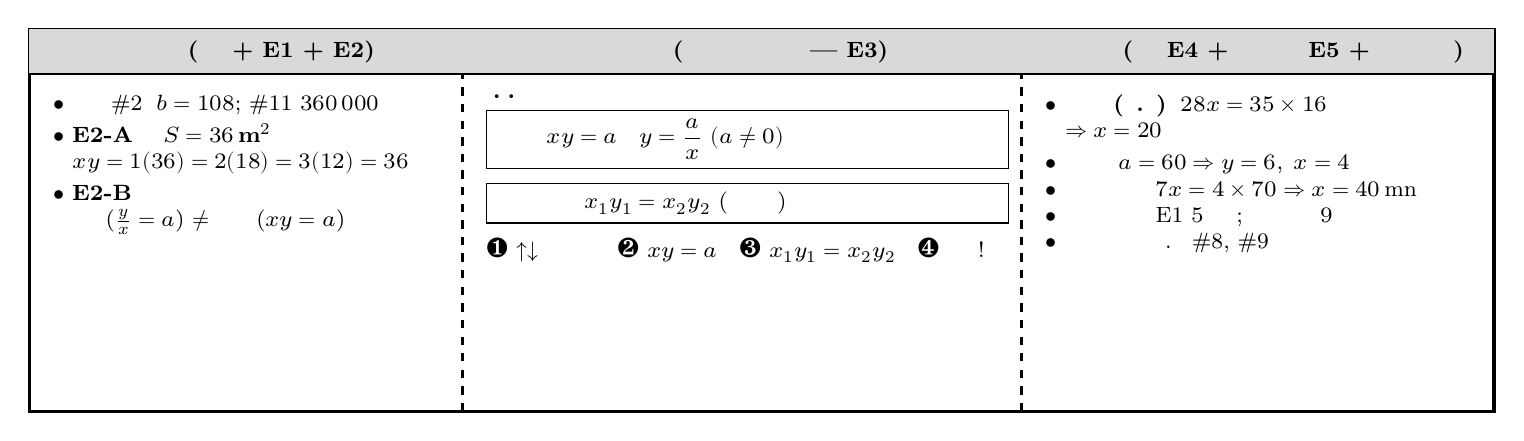
\begin{tikzpicture}[x=1cm, y=1cm, every node/.style={font=\footnotesize, text=black}]
  \draw[black, line width=1.2pt] (0,0) rectangle (18.6,4.85);
  \fill[headgray] (0,4.28) rectangle (18.6,4.85);
  \draw[black, line width=0.8pt] (0,4.28) -- (18.6,4.28);
  \draw[black, line width=0.85pt, dashed] (5.5,0) -- (5.5,4.28);
  \draw[black, line width=0.85pt, dashed] (12.6,0) -- (12.6,4.28);

  \node at (2.75,4.56) {\textbf{ផ្នែកឆ្វេង (កំណែ + \en{E1} + \en{E2})}};
  \node at (9.05,4.56) {\textbf{ផ្នែកកណ្ដាល (ខ្លឹមសារគោលរក្សាទុក — \en{E3})}};
  \node at (15.6,4.56) {\textbf{ផ្នែកស្ដាំ (គំរូ \en{E4} + ប្រតិបត្តិ \en{E5} + កិច្ចការផ្ទះ)}};

  \node[anchor=north west, align=left] at (0.18,4.14) {
    $\bullet$ \textbf{កំណែ៖} \#2ក $b=108$; \#11 $360\,000\riel$\\[2pt]
    $\bullet$ \textbf{\en{E2-A} ដី $S=36\unit{m}^2$៖}\\
    \hspace*{0.25cm}$xy = 1(36)=2(18)=3(12)=36$\\[2pt]
    $\bullet$ \textbf{\en{E2-B} ញែកប្រភេទ៖}\\
    \hspace*{0.25cm}ស្រប ($\frac{y}{x}=a$) $\neq$ ច្រាស ($xy=a$)
  };

  \node[anchor=north west, align=left] at (5.68,4.14) {
    {\muol\fontsize{8.4pt}{12pt}\selectfont ១\enbf{.}៣\enbf{.} ទំហំសមាមាត្រច្រាស}\\[3pt]
    \fbox{\parbox{6.4cm}{\textbf{ជាទូទៅ៖} $xy = a$ ឬ $y = \dfrac{a}{x}$ $(a\neq 0)$}}\\[4pt]
    \fbox{\parbox{6.4cm}{\textbf{វិបាកគូតម្លៃ៖} $x_1 y_1 = x_2 y_2$ (ផលគុណថេរ)}}\\[4pt]
    \cnum{1} $\uparrow\downarrow$ ផ្ទុយទិស \; \cnum{2} $xy=a$ \; \cnum{3} $x_1 y_1 = x_2 y_2$ \; \cnum{4} ផ្ទៀង!
  };

  \node[anchor=north west, align=left] at (12.78,4.14) {
    $\bullet$ \textbf{គំរូ ១ (ទំ.៣១)៖} $28x = 35\times 16$\\
    \hspace*{0.25cm}$\Rightarrow x = 20$ ថ្ងៃ\\[2pt]
    $\bullet$ \textbf{គំរូ ២៖} $a=60 \Rightarrow y=6,\; x=4$\\
    $\bullet$ \textbf{ប្រតិបត្តិ ១៖} $7x = 4\times 70 \Rightarrow x=40\unit{mn}$\\
    $\bullet$ \textbf{ប្រតិបត្តិ ២៖} \en{E1} $5$ ថ្ងៃ; ច្រូតស្រូវ $9$ ថ្ងៃ\\
    $\bullet$ \textbf{កិច្ចការផ្ទះ៖} ទំ.៤១ \#8, \#9
  };
\end{tikzpicture}
\end{center}

\secstrip{២. ចម្លើយផ្ទៀងផ្ទាត់រហ័សសម្រាប់សន្លឹកកិច្ចការសិស្ស (ទំព័រ ១ និង ទំព័រ ២)}{\en{Answer Key}}

\begin{tcolorbox}[
  enhanced, sharp corners, colback=white, colframe=black,
  boxrule=0.8pt, boxsep=1.5pt, top=3pt, bottom=3pt, left=5pt, right=5pt,
  after skip=3.5pt
]
  \fontsize{8.8pt}{13.2pt}\selectfont
  $\bullet$ \textbf{ផ្នែក \en{E1}៖} ត្រូវការតែ \textbf{$5$ ថ្ងៃ}; ចំនួនថ្ងៃត្រូវ\textbf{ថយចុះ} ។\\[2pt]
  $\bullet$ \textbf{ផ្នែក \en{E2}៖} \textbf{សកម្មភាព ១៖} បណ្ដោយ $y$: $\mathbf{12, 9, 6}$; ផលគុណ $xy$: $\mathbf{36, 36, 36, 36}$; តម្លៃ $y$ \textbf{ថយចុះ}; $xy = \mathbf{36},\; y=\mathbf{\frac{36}{x}}$ ។ \textbf{សកម្មភាព ២៖} (ក) $\frac{y}{x}=800 \to$ \textbf{ស្រប}; (ខ) $v\cdot t = 24 \to$ \textbf{ច្រាស}; (គ) $y-x=3 \to$ \textbf{មិនសមាមាត្រ} ។\\[2pt]
  $\bullet$ \textbf{ផ្នែក \en{E4}៖} \textbf{គំរូ ១៖} សមាមាត្រ\textbf{ច្រាស}; $28x = \mathbf{560} \implies x = \mathbf{20}$ ថ្ងៃ (ត្រូវធំជាង $16$ ថ្ងៃ) ។ \textbf{គំរូ ២៖} $a = \mathbf{60},\; y=\frac{60}{x}$; (ក) $y = \mathbf{6}$; (ខ) $15x=60 \implies x = \mathbf{4}$ ។\\[2pt]
  $\bullet$ \textbf{ផ្នែក \en{E5}៖} \textbf{១) រ៉ូប៊ីនេ៖} រយៈពេល\textbf{ថយចុះ}; $7x = 4\times 70 = 280 \implies x = \mathbf{40\unit{mn}}$ ។ \textbf{២) បិទ \en{E1}៖} $t = \mathbf{5}$ ថ្ងៃ; ច្រូតស្រូវ៖ $20x = 180 \implies x = \mathbf{9}$ ថ្ងៃ ។ \textbf{៣) វិនិច្ឆ័យ \en{A--D}៖} ជម្រើស \textbf{\en{C}} ។ \textbf{៤) សំបុត្រចេញ៖} (ក) $a = \mathbf{48}$; (ខ) $y = \mathbf{4}$ ។
\end{tcolorbox}

\secstrip{៣. ចម្លើយលម្អិតនៃកិច្ចការផ្ទះ (សម្រាប់ផ្ទៀងនៅដើមម៉ោងបន្ទាប់ ២.១--២.២)}{សៀវភៅគោល ទំ.៤១}

\begin{tcolorbox}[
  enhanced, sharp corners, colback=white, colframe=black,
  boxrule=0.8pt, boxsep=1.5pt, top=3pt, bottom=3pt, left=5pt, right=5pt
]
  \fontsize{8.7pt}{13.0pt}\selectfont
  $\bullet$ \textbf{\#8 (ទំ.៤១)៖} ដោយចំនួនកម្មករ ($25$ នាក់) រក្សានៅដដែល នោះចំនួនម៉ោងធ្វើការ $t$ និងចំនួនស្បែកជើងជា\textbf{ទំហំសមាមាត្រស្រប}៖ $\dfrac{t}{450} = \dfrac{26}{1\,300} = \dfrac{1}{50} \implies t = \dfrac{450}{50} = \mathbf{9\text{ ម៉ោង}}$ ។\\[3pt]
  $\bullet$ \textbf{\#9 (ទំ.៤១)៖} តាង $x$ ជាចំនួនម៉ោងក្នុង ១ ថ្ងៃដែលកម្មការិនី $16$ នាក់ត្រូវធ្វើការក្នុងរយៈពេល $16$ ថ្ងៃ ។ ដោយបរិមាណការងារសរុបថេរ គេបានផលគុណម៉ោងកម្មករសរុបស្មើគ្នា៖ $16 \times x \times 16 = 12 \times 7 \times 8 \implies 256x = 672 \implies x = \dfrac{672}{256} = \mathbf{\dfrac{21}{8}\text{ ម៉ោង}} = \mathbf{2\dfrac{5}{8}\text{ ម៉ោង}} = \mathbf{2.625\text{ ម៉ោង}}$ ($2$ ម៉ោង $37$ នាទី $30$ វិនាទី) ។
\end{tcolorbox}

\end{document}
